\documentclass[10pt]{article}
\usepackage{graphicx}
\usepackage[margin=1.5cm]{geometry}
\usepackage{amsmath}
\def\brcurs{{\mbox{$\resizebox{.16in}{.08in}{
\includegraphics{BoldR}}$}}}
\def\rcurs{{\mbox{$\resizebox{.16in}{.08in}{
\includegraphics{ScriptR}}$}}}

\begin{document}
\twocolumn

\title{Thursday Warm-up: Magnetic Vector Potential and Magnetic Dipoles}
\author{Prof. Jordan C. Hanson}

\maketitle

\begin{figure}
\centering
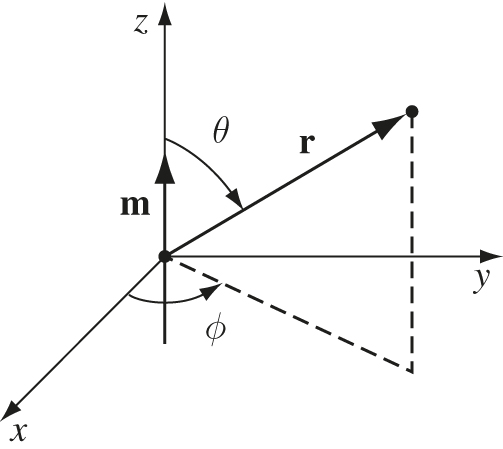
\includegraphics[width=0.20\textwidth]{figures/5_57.jpg}
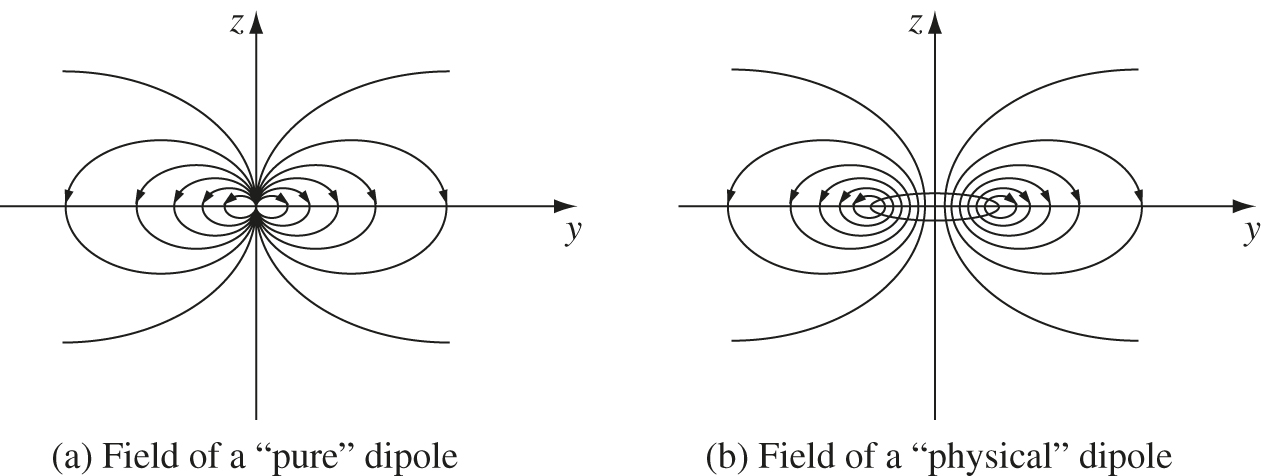
\includegraphics[width=0.28\textwidth,trim=5cm 0.5cm 0cm 0cm,clip=true]{figures/5_58.jpg}
\caption{\label{fig:1} (Left) A magnetic dipole moment oriented along the z-axis. (Right) The $\mathbf{B}$-field of a magnetic dipole.}
\end{figure}

\section{Memory Bank}

\begin{itemize}
\item \textbf{Magnetic vector potential}:
\begin{equation}
\mathbf{B} = \nabla \times \mathbf{A}
\end{equation}
\item \textbf{Magnetic flux and vector potential:}
\begin{equation}
\Phi_{\rm B} = \int \mathbf{B} \cdot d\mathbf{a} = \oint \mathbf{A} \cdot d\mathbf{l}
\end{equation}
\item Curl in spherical coordinates, $\mathbf{A}(r,\theta) = A(r,\theta)\hat{\boldsymbol{\phi}}$
\begin{equation}
\nabla \times \mathbf{A} = \frac{1}{r\sin\theta}\left(\frac{\partial}{\partial\theta}(\sin\theta A_{\phi} \right) - \frac{1}{r}\left(\frac{\partial}{\partial r} (r A_{\phi})\right)\hat{\boldsymbol{\theta}}
\end{equation}
\end{itemize}

\vspace{2cm}

\section{Magnetic Vector Potential and \\ Magnetic Dipoles}

\begin{enumerate}
\item The magnetic dipole moment of a loop of current is define like:
\begin{equation}
\mathbf{m} = I\int d\mathbf{a}
\end{equation}
(a) Suppose a circular loop of current with radius $b$ lies in the xy-plane, centered at the origin (Fig. \ref{fig:1}).  Calculate $\mathbf{m}$. (b) According to the multipole expansion of the magnetic vector potential, the dipole component of the vector potential is
\begin{equation}
\mathbf{A}_{\rm dip} = \frac{\mu_0}{4\pi}\frac{\mathbf{m}\times \hat{\mathbf{r}}}{r^2}
\end{equation}
Express the vector potential as a function of $r$ and $\theta$. \\ \vspace{4cm}
\item (a) Calculate the $\mathbf{B}$-field of the dipole in Fig. \ref{fig:1}, using the curl in spherical coordinates. (b) Sketch the dipole field, and show that it has the structure of an electric dipole field (Fig. \ref{fig:1}). \\ \vspace{4cm}
\item Suppose a square loop of current with side length $d$ lies in the xy-plane centered at the origin, in the presence of a uniform $\mathbf{B}$-field in the $\hat{\mathbf{x}}$ direction. (a) What is the magnetic dipole moment, $\mathbf{m}$? (b) Show that the torque on the loop is 
\begin{equation}
\mathbf{N} = \mathbf{m} \times \mathbf{B}
\end{equation}
\end{enumerate}

\end{document}
